\chapter{Design}
\todo{short introduction to what will be addressed in this chapter}

\subsection{Concept}
The concept of the product is to be able to apply voice effects in real-time without having to turn to a panel or having someone do it for you. 

A thing most singers almost always have available are their hands. Therefore a device controlled by the hands movements seems the obvious choice.

The device will implement a gyroscope to sense the movements of the hand.

The device then needs to be told that an effect has been initiated. This is done by connecting the thumb to the finger in control of the desired effect.

When this has been done the gesture to apply the effects is done. 

\begin{itemize}
\item Harmonising: This will be controlled by turning the hand while having thumb and a finger pressed together, like turning a knob or volume control.
\item Pitch: This will be controlled by lifting or lowering the hand while having thumb and a finger pressed together, like pulling a slider up or down.
\end{itemize}

\begin{figure}[!h]
\centering
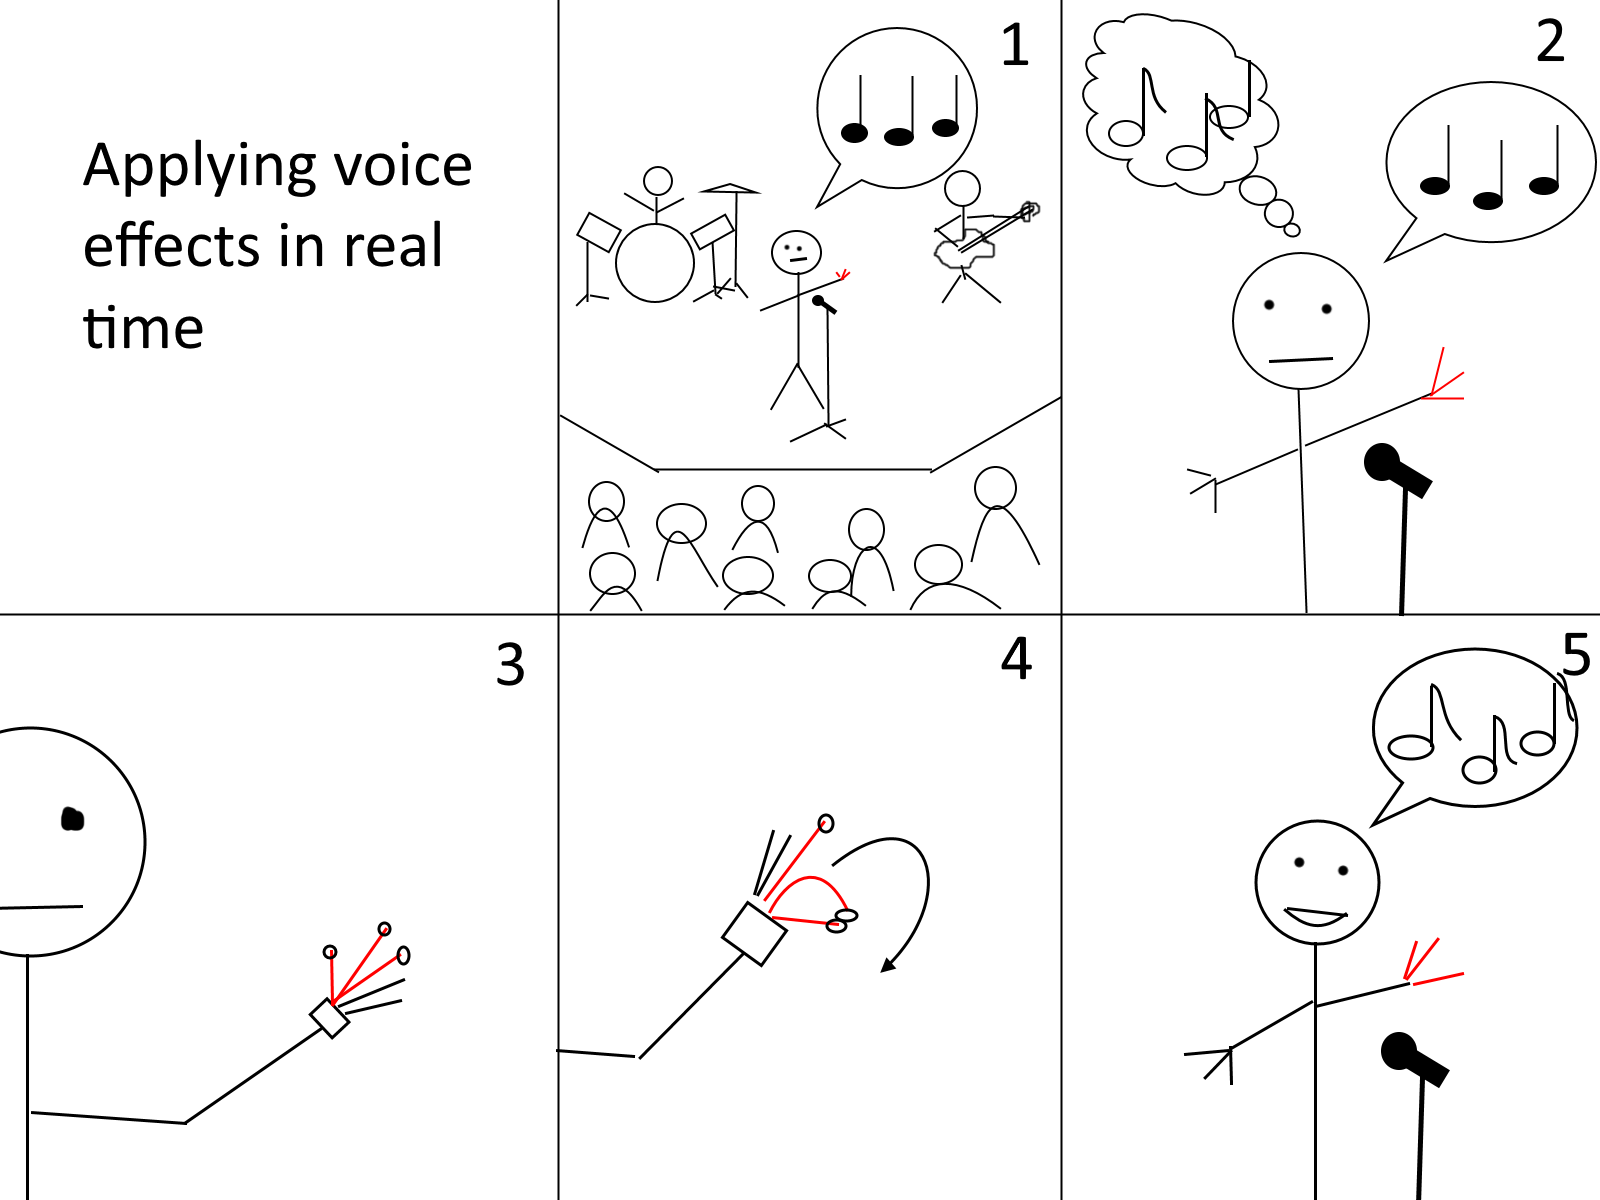
\includegraphics[scale=0.3]{Storyboard2}
\caption{The storyboard.} \label{Storyboard1}
\end{figure}

\todo{insert storyboard here, when a nice looking one has been made}

\subsection{Sketching}
\begin{figure}[!h]
\centering
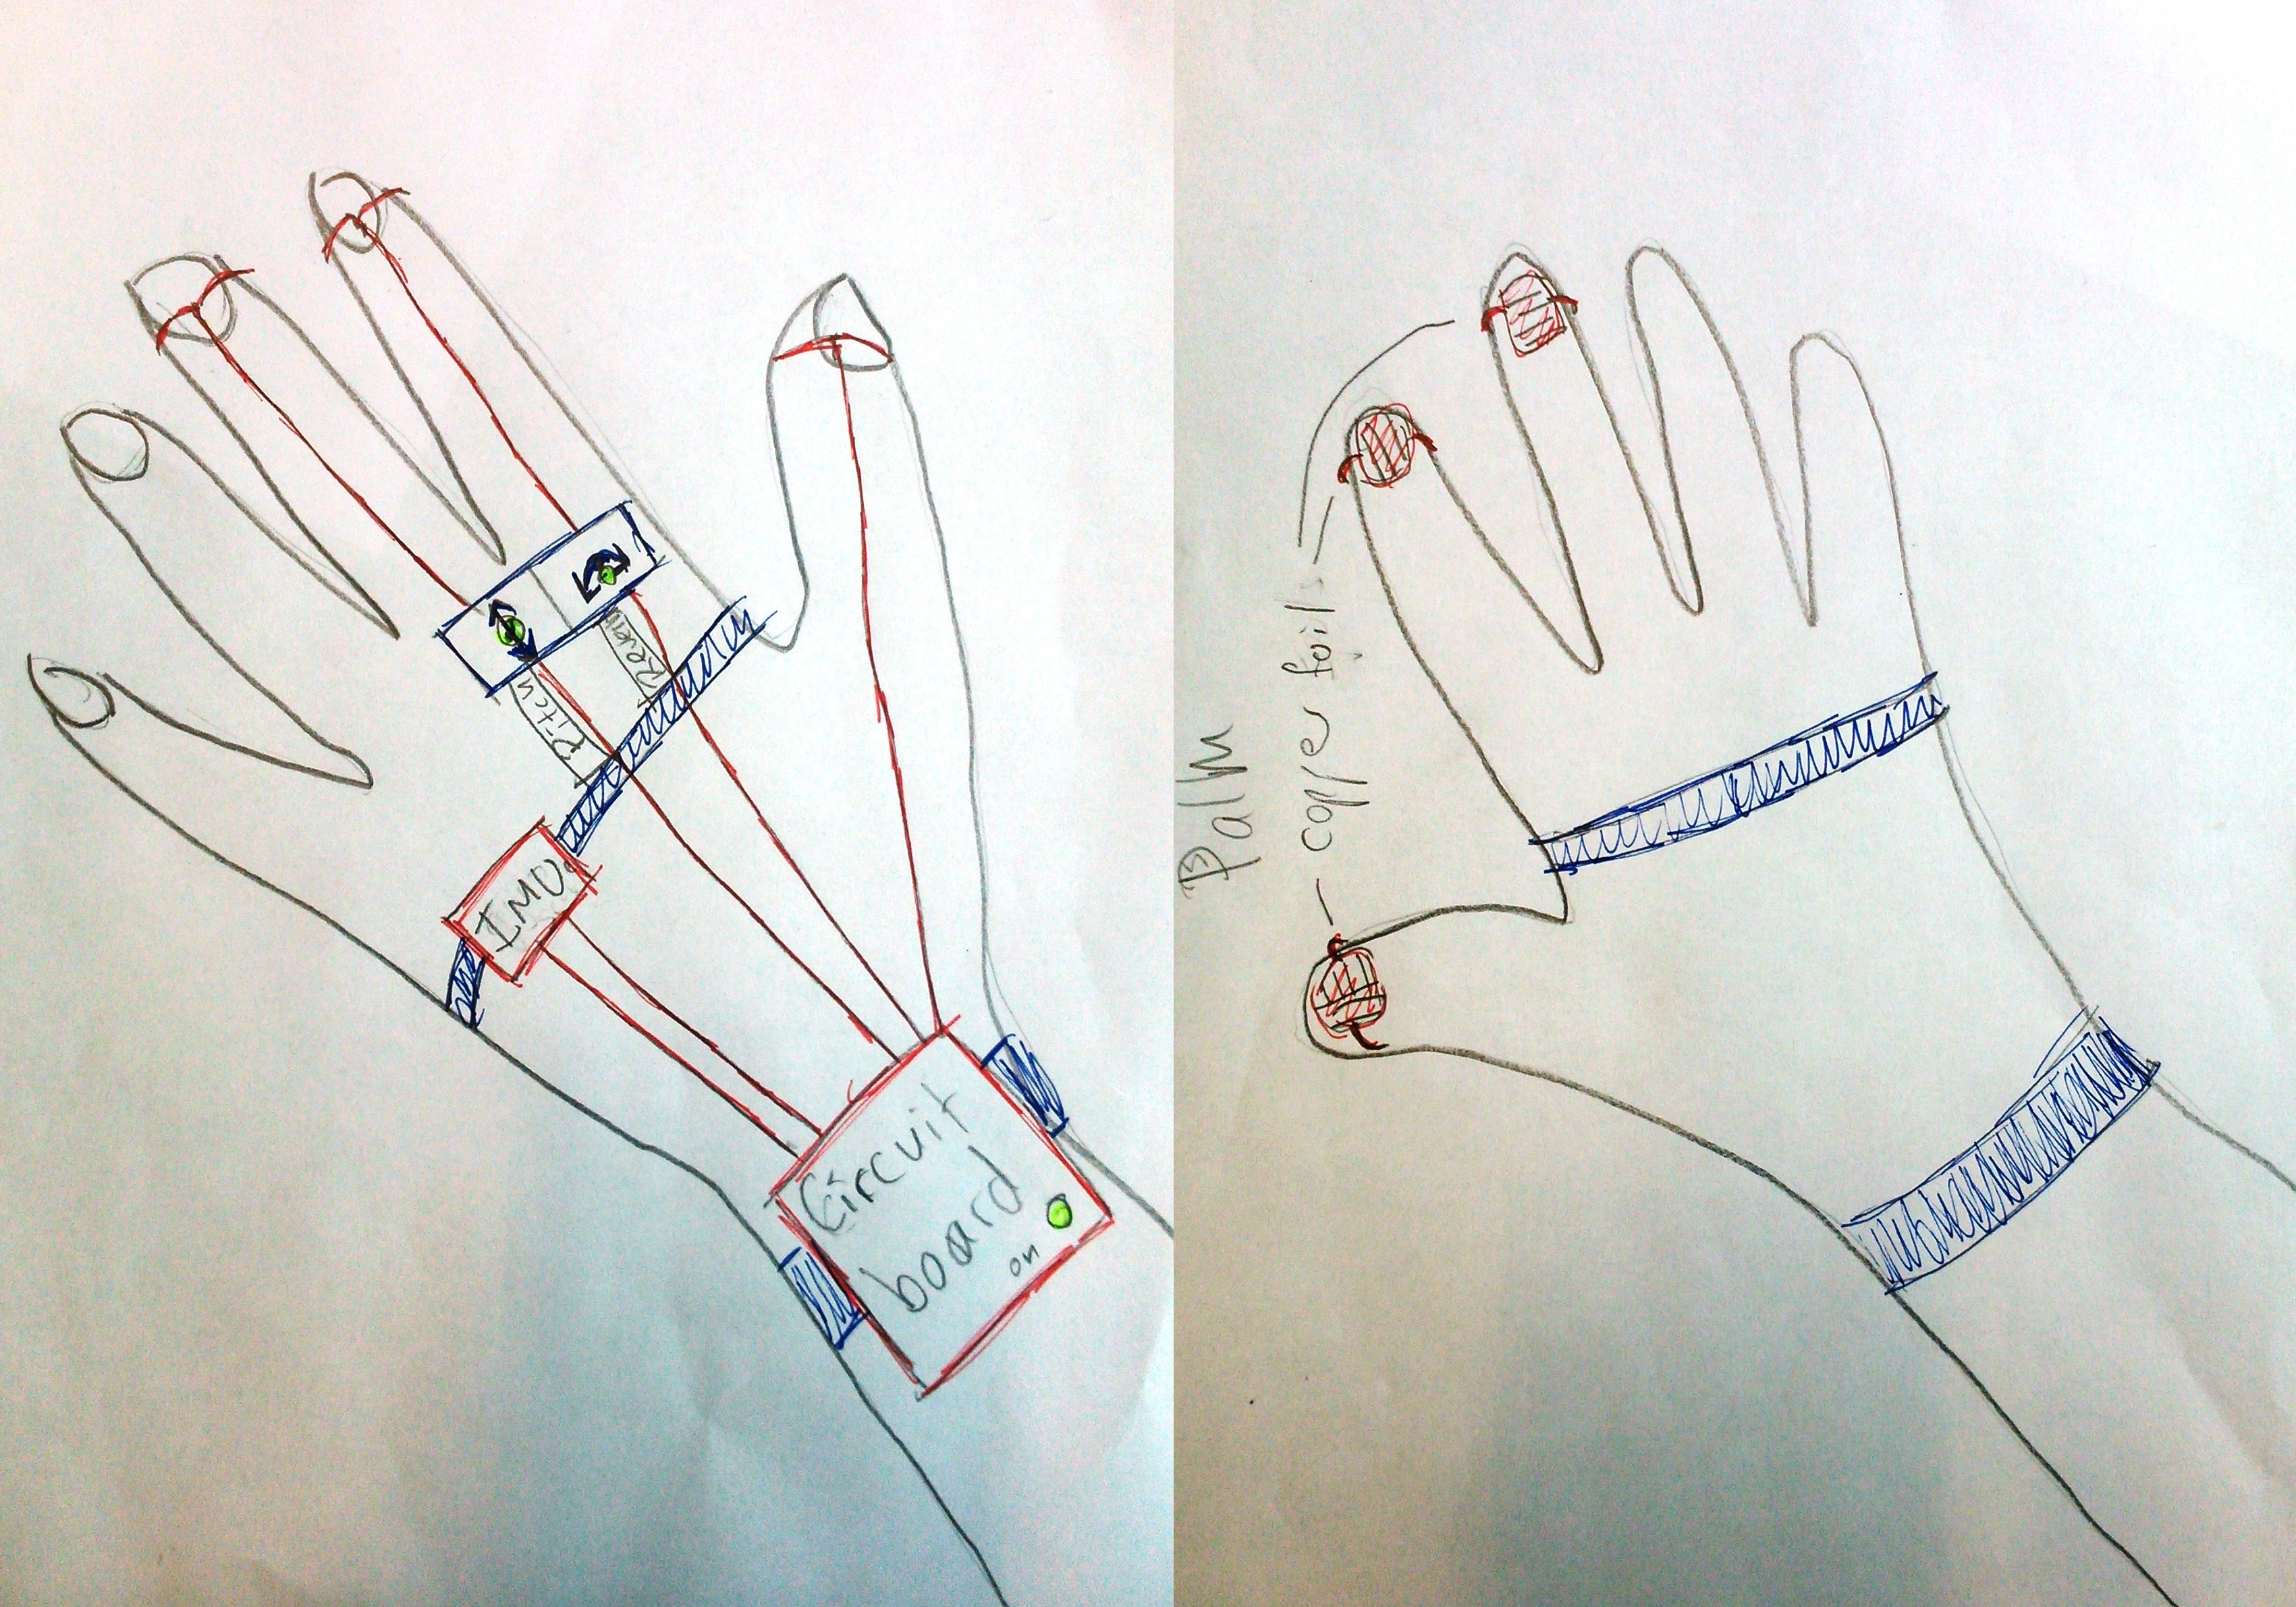
\includegraphics[scale=0.1]{Sketch1}
\caption{The first sketch} \label{Sketch1}
\end{figure}

The first sketch and the first concrete design of the device have copper foil on thumb, index finger and middle finger. 

On the knuckles there are illustrations of the gestures, that you are supposed to do to manipulate the effects. Beneath those are small labels with the effect name. In this design reverb was used instead of harmonising. This was later changed, since reverb is not manipulated quite as much as harmonising. 

The sensor is attached to the hand by a velcro strip as is the circuit board. 

A quick informal test with three participants was conducted and they were told what the drawing was supposed to be and what it should do. They then had to figure out based on the sketch how to do those things. 
\begin{itemize}
	\item One thing made very clear was that they all had difficulty figuring out how to get to the activate stage. None of them connected their fingers.
	\item Most figured out which type of gesture in general had to be done but they were missing the finger connections which made the gestures wrong
	\item They all found out which finger created which effect
\end{itemize}

Based on this the next focus will be on creating some feedforward and perceived affordance that tell the user that to activate the glove you need to connect two fingers.

The second sketch changed the illustrations since people had a hard time performing the correct gestures with the old ones.

\begin{figure}[!h]
\centering
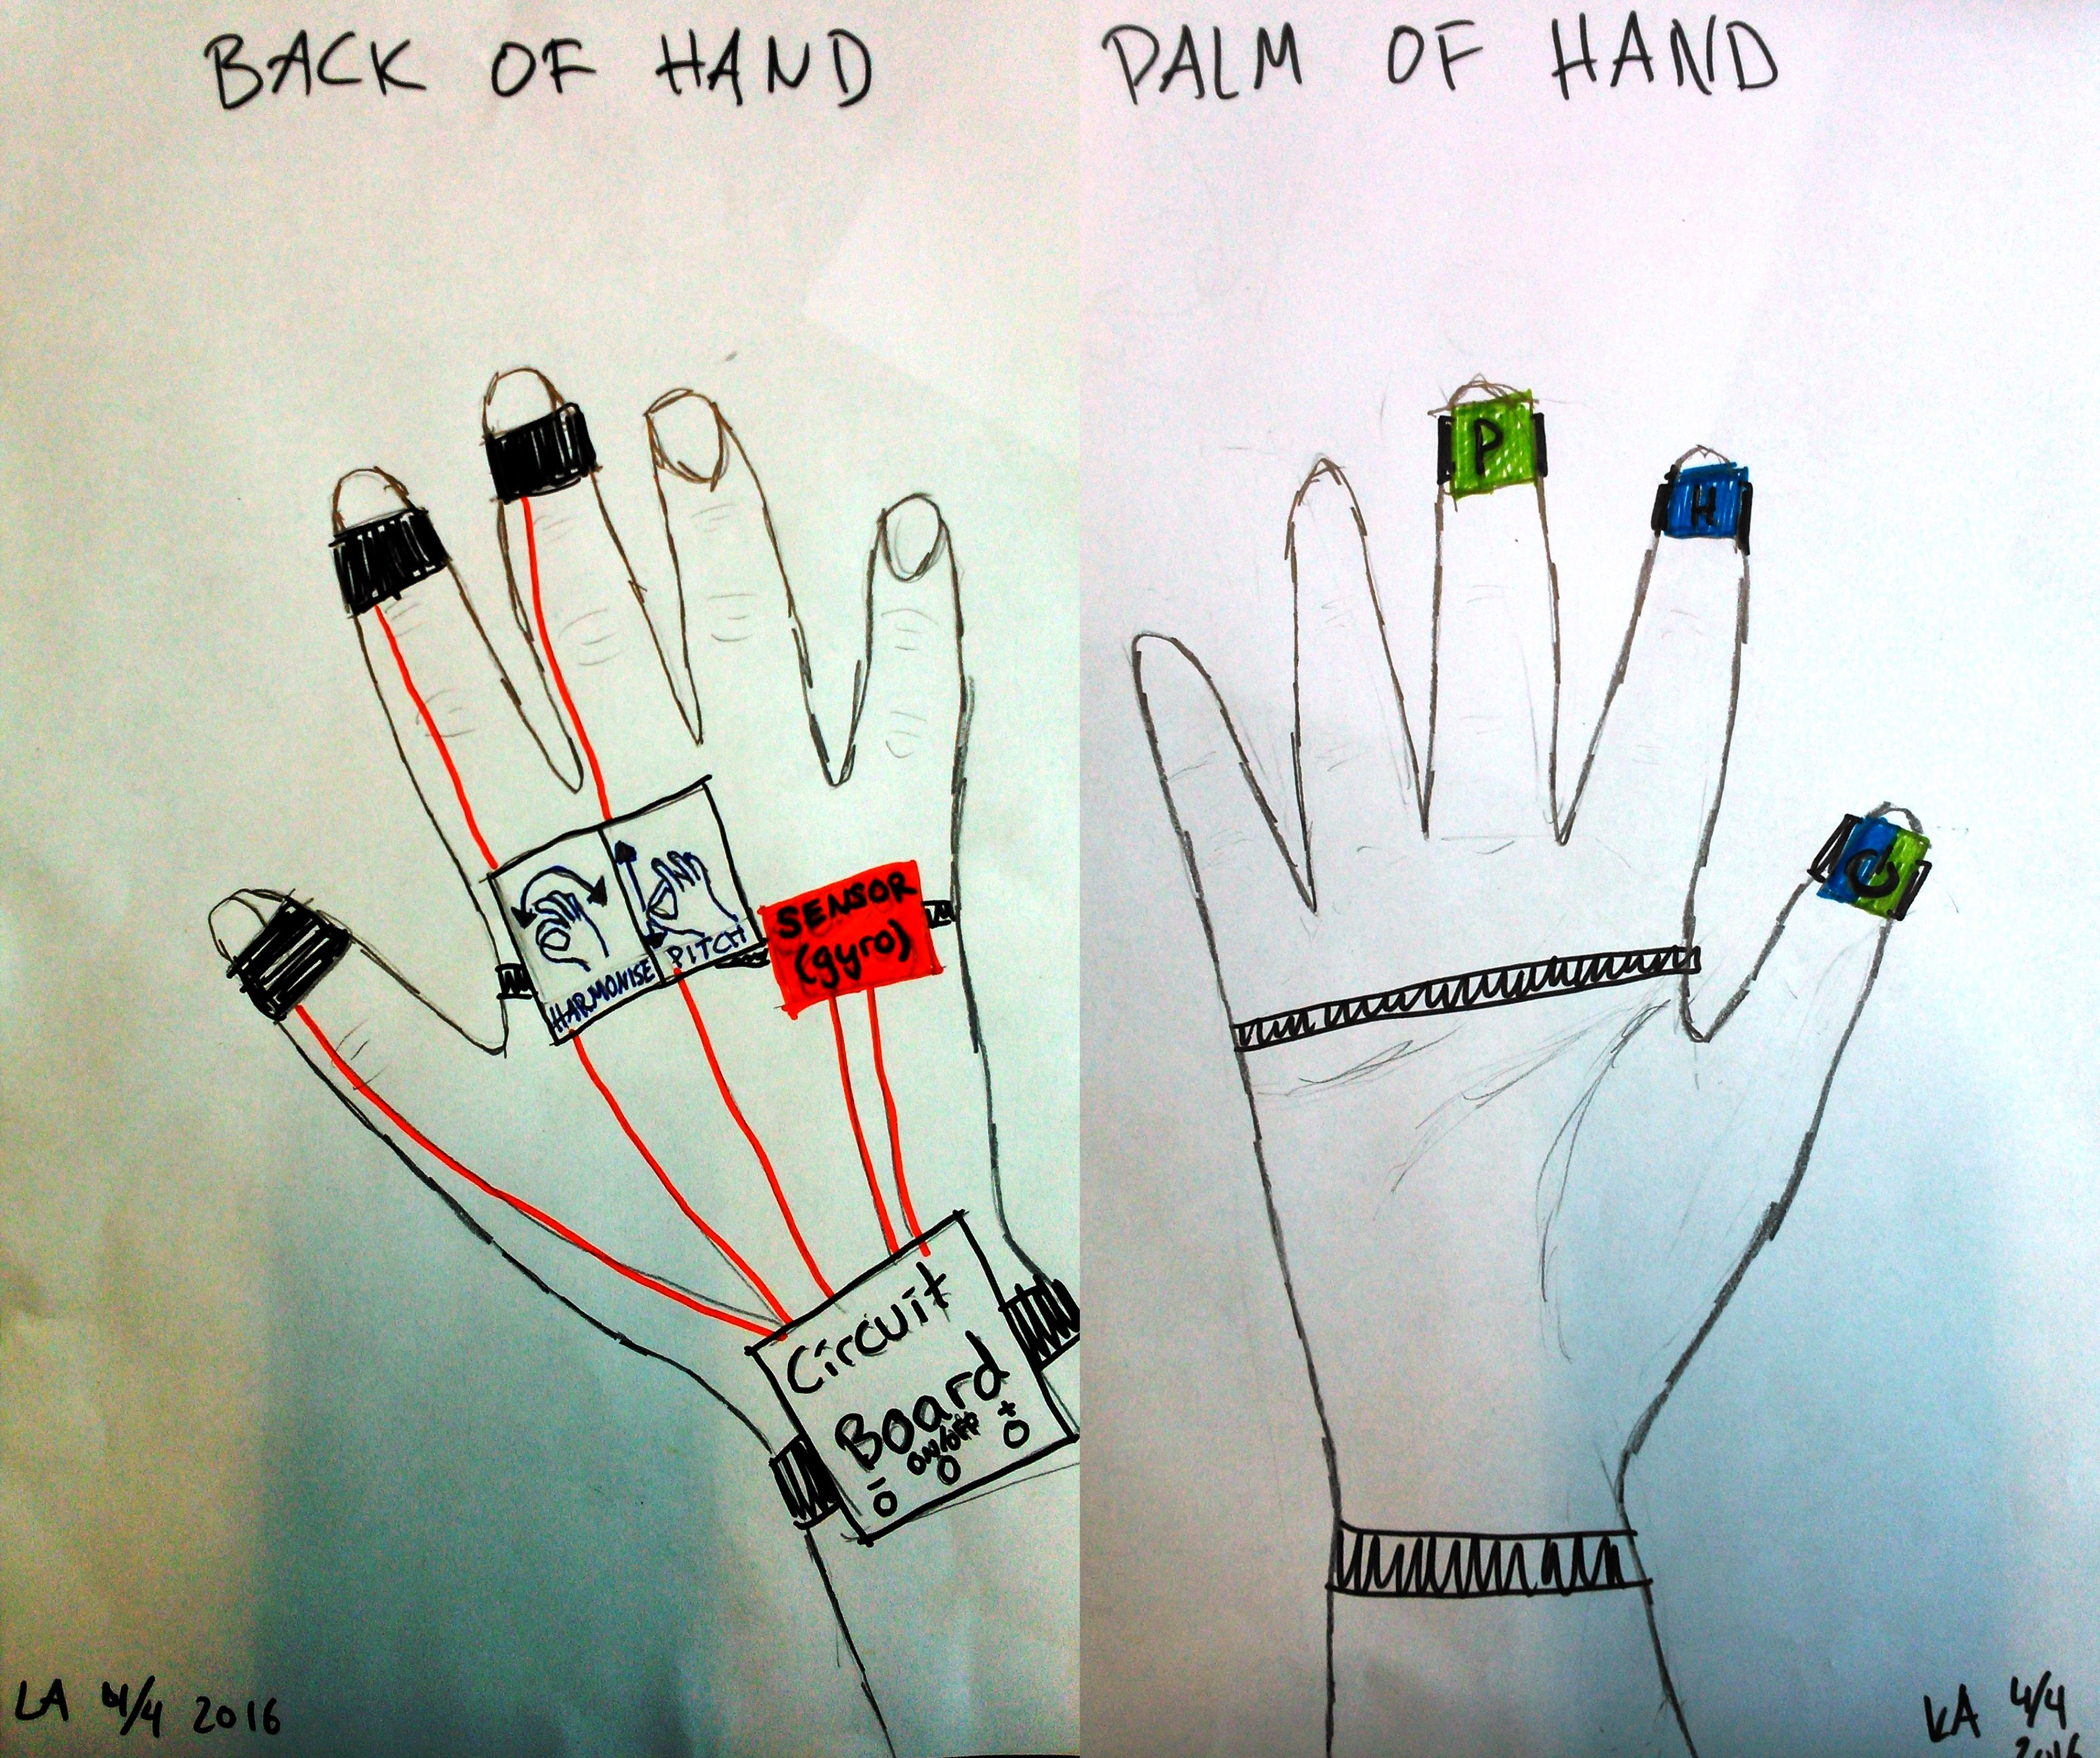
\includegraphics[scale=0.1]{Sketch2}
\caption{The second sketch} \label{Sketch2}
\end{figure}

Colour was also added to the copper foil, a different one on the index and middle finger and then both on the thumb. This was done to create a connection between fingers and thumb.

LEDs were added to create some feedback on the actions.

An quick informal test was done with two participants with the revised sketch. Now there were a better indication that one needed to connect two fingers, but not anything that indicated that they needed to stay connected.
\begin{itemize}
	\item One suggested that instead of on/off LED maybe a connected/not connected LED.
	\item The arrows were found to be confusing for one tester.
	\item Another tester easily understood the pitch action but was a bit confused with the placement of the arrow on the harmonise action.
	\item The dual colour on the thumb suggested that both actions could be done at the same time.
	\item The plus and minus LEDs confused one tester, but this could also be because the drawing was unclear.
\end{itemize}

